\chapter{Experiments}

In this chapter we assess the representations obtained by minimising the Variational-InfoNCE loss and compare results against its non-variational counterpart. We train the encoders on sequential data from the audio domain and assess the quality of the representations. The assessment is achieved by transforming the latent space into a two-dimensional space using t-SNE and observing clusters. Additionally, the representations obtained from the encoders are used as input for a linear classifier, whose accuracy scores provide insights in the representations' performance.

Additionally, we gather more insights in the representations. We assess the required amount of labelled data required for obtaining adequate performance in downstream tasks, by training the linear classifier on smaller subsets of the dataset. Finally, we provide insights in the interpretation of the latent features, by developing a decoder for the representations. We can then observe the information that is contained in each of the representation's components by altering values and observing the produced output of the decoder. 


%- Experimental details encoder:
%	- Learning task: to find representations for speech data.
%	- Dataset:
%		- full data + split up
%	- Architecture
%- Results
%	- Loss functies
%	- Linear separability (t-sne)
%	
%- Generalisation (generalisation)
%		- Accuracies Subsets
%- Interpretability
%		- Encoder distributions (shows that interpolation can make sense)
%		- Decoder: loss, architecture

	






% TODO: I CALL IT Variational Greedy Infomax: V-GIM

\section{Experimental details encoder}

	
	
	\subsection{Dataset}
		The Greedy Infomax model is trained on speech data. The model takes as input a raw speech signal of a fixed length and outputs a latent representation for that signal. The dataset is split up into 729 training files and 122 test files. In each file consists of a single spoken sound consisting of three consonants and three vowels, where the consonants and vowels alternate each other. Some Examples are the sounds "gi-ga-bu" and "ba-bi-gu". All the sounds are spoken by the same person, at a constant and peaceful \textbf{todo: describe emotional aspects of speech audio}. 
		
		The following transformations are applied to the audio files. Although the original contains a sample rate of 441 Khz, the audio files are downsampled to 16 Khz, matching the sample rate used by Löwe \cite{lowePuttingEndEndtoEnd2020}. This significantly reduces the size of the latent representations, and thus the required amount of VRAM during training. Additionally, two types of noise are added to the data. We apply Gaussian white noise, at different decibels ranging between zero and fifteen \textbf{TODO ...}.
		
		- also background noise from dataset. is a way to enlarge our dataset. 
		- Each audio file is cut to have length \textbf{10240}. Additionally, 
		
		
		Splitting: see appendix  \ref{appendix:split_syllables}
		
	\subsection{Architecture}
		% cnn + gru: so inputs can have variable lengths
			Training is done speech signals of fixed length, eg 8,800 samples. Notice however, that the neural network only makes use of convolutional neural networks layers and GRU's, no fully connected layers. The input dimensions can therefore be variable during inference. Only the number of channels in the latent representations should be constant, but the length can change.
			
		\begin{figure}[h]
			\centering
			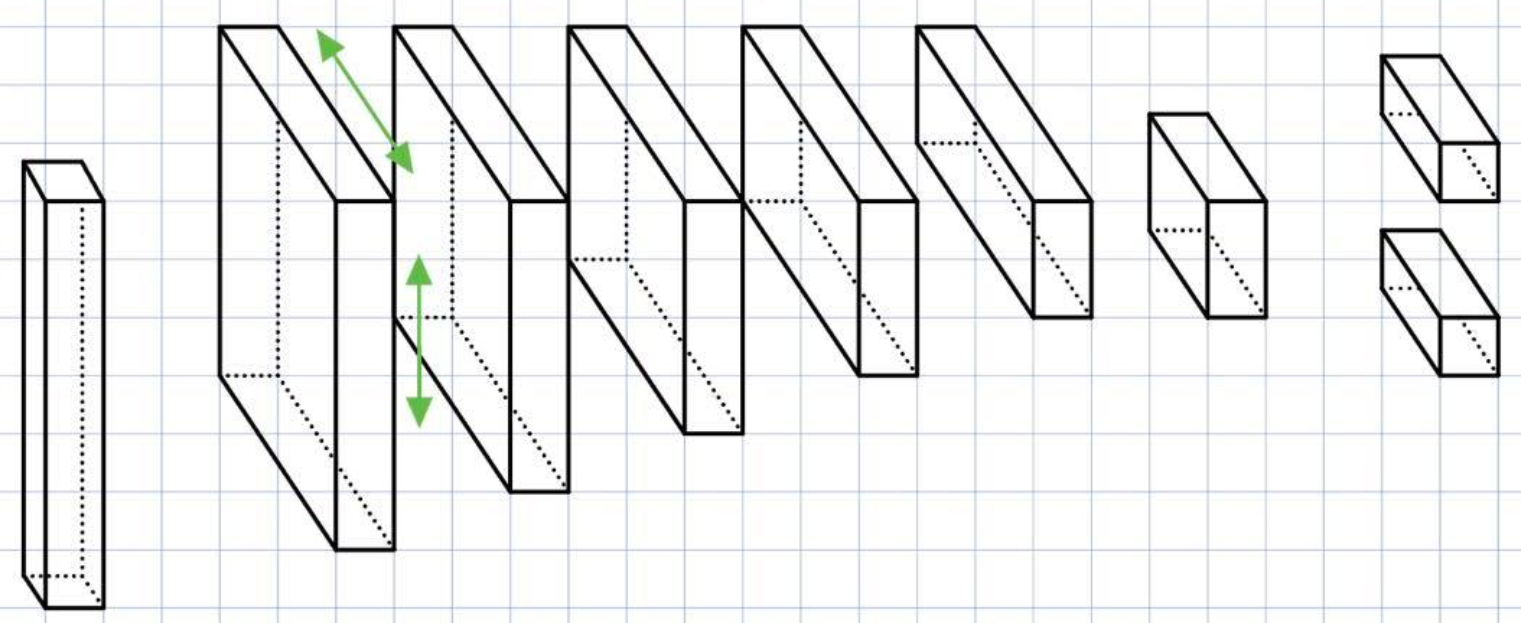
\includegraphics[width=0.7\linewidth]{architecture}
			\caption{}
			\label{fig:architecture}
		\end{figure}
	
		Figure \ref{fig:architecture} displays how via contrastive predictive coding an input speech signal is transformed into two latent vectors. The two vectors combined describe a Gaussian distribution for each feature of the latent representation. One vector corresponds to the means and the other to the standard deviations of the latent distributions. We variational autoencoders assume independent latent features, such that the covariance matrix is non negative on the diagonal and zero off the diagonal. This allows the covariance matrix to be discribed using a single vector. We again, make use of this (plausible incorrect?) assumption of having independent latent features.




		% Training on longer patches, classification on padded sub-patches.
		During inference, (in this context obtaining the latent representations for our input signals), depending on the length of the input signal, the length of the output latent representation will differ.
		If we wish to look at how separable latent representations are for syllables, the length can be variable. Some input sounds could be 6,600 samples, while others 8,800 samples. We therefore pad the syllables with zeroes in front and end of the signal, to obtain fixed length of equal to that of the longest syllable; 8,800 samples.
		
		Training happens on longer data samples, and every \textbf{X} epochs t-SNE visualisations are made to observe evolutional of dis-entanglement.
		

\section{Results}

	% Enkele loss curces etc
	\subsection{Results CPC Simple v2 w/ 2 modules}
	
	\subsection{Distributions}
	
	% loss func only shows part of picture -> towards tsne
		Although loss is used as evaluation metric, it only shows part of the picture. The main objective for the representations is to obtain some form of "decoupled/dis-entanged" features that are more easily separable. This evaluation is done by projecting the latent representations to a 2D plane, via t-SNE. Then datapoints are coloured in depending on their the syllable that was pronounced, eg: "gi" or "ga".
		
		
		

		%Graphs t-sne: Beta = 0	
		%	\begin{figure}[h]
		%		\centering
		%		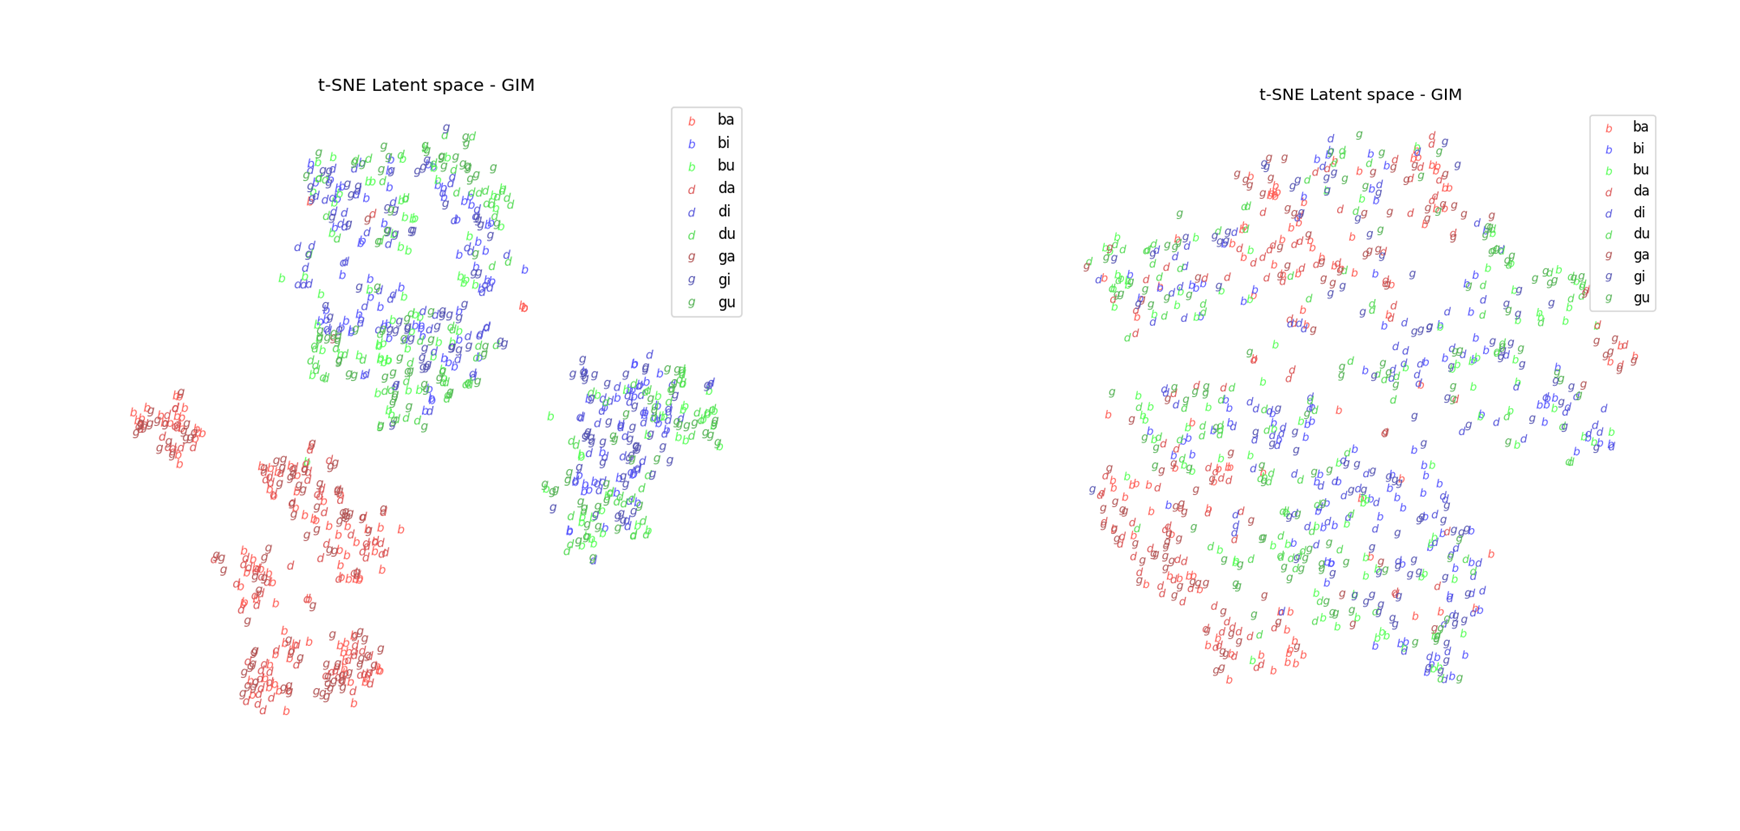
\includegraphics[width=0.7\linewidth]{screenshot023}
		%		\caption{}
		%		\label{fig:tsne_two_module_kld_0}
		%	\end{figure}
		%	
		%	
		%	\begin{figure}[h]
		%		\centering
		%		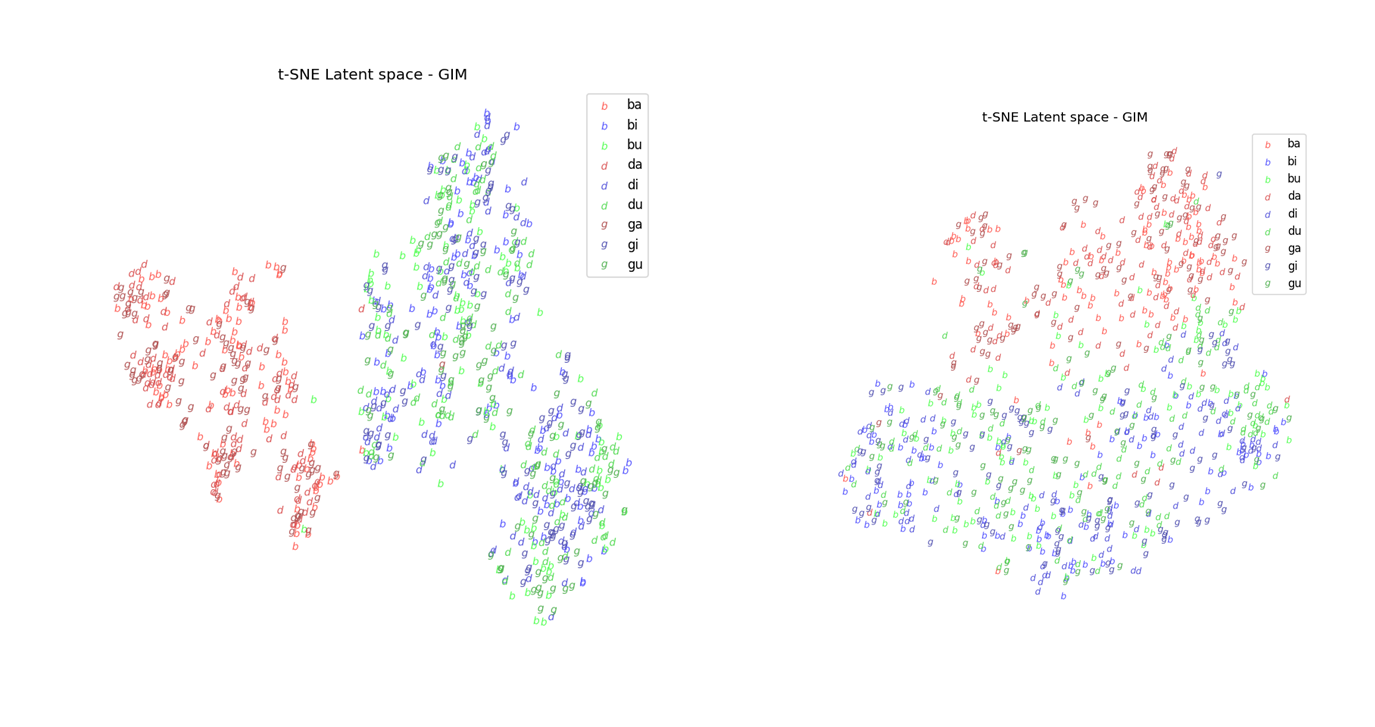
\includegraphics[width=0.7\linewidth]{screenshot024}
		%		\caption{}
		%		\label{fig:tsne_two_module_kld_0033}
		%	\end{figure}
	
	%	
	%	\ref{fig:tsne_two_module_kld_0}: can see that second model harms performance. We believe this can be explained via the learning rate. \ref{fig:tsne_two_module_kld_0033}, there we see that second module performs better separation, indicating that the intermediate KL convergence constraint (causing the normal Gaussian distributions) also serves as a batch normalisation term, and thus resulting in faster convergence.
	%
	%	
	%	---------------------------------------------
	%	
	%	\textbf{T-sne visualisations:}
	%	Multiple models trained, trained GIM, but single module (exact CPC architecture), one with autoregressor and once without autoregressor layer, so only CNN layers. 200 epochs, trained on split up data samples.
	%	
	%	1) Only CNN: We observe better linear separability
	%	\begin{figure}[h]
	%		\centering
	%		\includegraphics[width=0.7\linewidth]{"cpc architecture ONLY CNN t-SNE_latent_space_GIM"}
	%		\caption{}
	%		\label{fig:cpc-architecture-only-cnn-t-snelatentspacegim}
	%	\end{figure}
	%	
	%	2) CNN + 1 autoregressor layer:
	%	\begin{figure}[h]
	%		\centering
	%		\includegraphics[width=0.7\linewidth]{"cpc architecture CNN + GRU t-SNE_latent_space_GIM"}
	%		\caption{}
	%		\label{fig:cpc-architecture-cnn--gru-t-snelatentspacegim}
	%	\end{figure}
	%	
	%	3) This is the pure data visualised (no latent representation).
	%	Were at least doing a bit better than the original data, so that's good! our work is not for nothing.
	%	\begin{figure}[h]
	%		\centering
	%		\includegraphics[width=0.7\linewidth]{"_ t-SNE_latent_space_Original data"}
	%		\caption{}
	%		\label{fig:-t-snelatentspaceoriginal-data}
	%	\end{figure}
	%	
	%	
	%	4) old GIM with all modules each one layer. l1 .. 5 - cnn, l6 = gru. img shows l5 = cnn:
	%	model can more easily distinguish A's from other \textbf{klinkers}. Partly, it kinda makes sense for GIM to learn to separate \textbf{klinkers}. Since they last longer (longer duration), the loss function will more likely randomly sample a subwindow from the "aa's" than from the \textbf{medeklinker} part.
	%	
	
	
	
	
	
	
	
	
	
	
	

%		\begin{figure}
%			\centering
%			\includegraphics[width=0.7\linewidth]{"t-sne kld=0 module 2"}
%			\caption{}
%			\label{fig:t-sne-kld0-module-2}
%		\end{figure}
%		\begin{figure}
%			\centering
%			\includegraphics[width=0.7\linewidth]{"t-sne kld=0.0033 module 1"}
%			\caption{}
%			\label{fig:t-sne-kld0}
%		\end{figure}
%		\begin{figure}
%			\centering
%			\includegraphics[width=0.7\linewidth]{"t-sne kld=0.0033 module 2"}
%			\caption{}
%			\label{fig:t-sne-kld0}
%		\end{figure}
%		\begin{figure}
%			\centering
%			\includegraphics[width=0.7\linewidth]{"t-sne kld=0 module 1"}
%			\caption{}
%			\label{fig:t-sne-kld0-module-1}
%		\end{figure}
	
	
	\subsubsection{T-sne}
	T-distributed stochastic neighbour embedding.
	
	
	Visualising data using T-sne.
	given N high-dimensional objects x1 .. xN. wants to see underlying structure of the data. eg clusters? local structures?
	
	How visiualise very high dimensional data?
	
	Introduction:
		build map where similar data points are moved close to each other and unsimilar points far away. and map in eg 2 or 3 dims. (scatter plot).
		
		minimize some objective function:
			eg PCA. finds linear projection of high dim data st variance of projected data is maximised.
	
	tsne:
		measure similarity between points, only look at local similarities.
		\begin{figure}[h]
			\centering
			\includegraphics[width=0.7\linewidth]{"tsne gaus"}
			\caption{}
			\label{fig:tsne-gaus}
		\end{figure}
		
		i = current point. j = other point.
		fraction is normalisation.
		
		-> pij = pdf which measures similarity between points i and j.
		if two points are similar: pij = large, dissimimlar: infinitessimal.
		$$
		p_{i j}=\frac{\exp \left(-\left\|\mathbf{x}_i-\mathbf{x}_j\right\|^2 / 2 \sigma^2\right)}{\sum_k \sum_{l \neq k} \exp \left(-\left\|\mathbf{x}_k-\mathbf{x}_l\right\|^2 / 2 \sigma^2\right)}
		$$
		
		t-Distributed Stochastic Neighbor Embedding
		- In practice, we compute the input similarities slightly differently:
		$$
		p_{j \mid i}=\frac{\exp \left(-\left\|\mathbf{x}_i-\mathbf{x}_j\right\|^2 / 2 \sigma_i^2\right)}{\sum_{j^{\prime} \neq i} \exp \left(-\left\|\mathbf{x}_i-\mathbf{x}_{j^{\prime}}\right\|^2 / 2 \sigma_i^2\right)}
		$$
		- We set the bandwidth $\sigma_i$ such that the conditional has a fixed perplexity
		- Finally, we symmetrize the conditionals: $p_{i j}=\frac{p_{j \mid i}+p_{i \mid j}}{2 N}$
		
		not joint distr, but conditional. only bottom part has changed, so only points that invole point xi.
		allows to set different bandwidth sigmai.
			such that different parts in dataset may have diff densities and fixes that.
			
			
		
		must layout points in map. Move points around to minimize: $K L(P \| Q)=\sum_i \sum_{j \neq i} p_{i j} \log \frac{p_{i j}}{q_{i j}}$
		
		will do gradient descent in kull bach leibler divergence such that kl becomes small.
			
			- Large $p_{i j}$ modeled by small $q_{i j}$ ? Big penalty!
			- Small $p_{i j \text { modeled by large }} q_{i j}$ ? Small penalty!
			- Hence, t-SNE mainly preserves local similarity structure of the data
				because small penality: doesnt care for points that are far apart. (only checks local similarity)
				
		doesn't use gaussian kernel! instead uses student t distribution.
		a lot more heavy tailed than gaussian distribution.
			
			
		Why a Student-t distribution?
		- Why do we define map similarities as $q_{i j} \propto\left(1+\left\|\mathbf{y}_i-\mathbf{y}_j\right\|^2\right)^{-1}$ ?
		- Suppose data is intrinsically high-dimensional
		- We try to model the local structure of this data in the map
		- Result: dissimilar points have to be modeled as too far apart in the map!
		t-sne allows that to happen.
		
		
		
		
		
		
	

			
			\begin{figure}[ht] % four t-sne images
				\centering
				\begin{subfigure}{0.45\linewidth}
					\centering
					\includegraphics[width=\linewidth]{"t-sne kld=0.0033 module 1"}
					\caption{}
					\label{fig:t-sne-kld33-module1}
				\end{subfigure}
				\hspace{0cm}
				\begin{subfigure}{0.45\linewidth}
					\centering
					\includegraphics[width=\linewidth]{"t-sne kld=0.0033 module 2"}
					\caption{}
					\label{fig:t-sne-kld33-module2}
				\end{subfigure}
				\vspace{0cm}
				\begin{subfigure}{0.45\linewidth}
					\centering					
					\includegraphics[width=\linewidth]{"t-sne kld=0 module 1"}
					\caption{}
					\label{fig:t-sne-kld0-module-1}
				\end{subfigure}
				\hspace{0cm}
				\begin{subfigure}{0.45\linewidth}
					\centering
					\includegraphics[width=\linewidth]{"t-sne kld=0 module 2"}
					\caption{}
					\label{fig:t-sne-kld0-module-2}
				\end{subfigure}
				\caption{My images}
				\label{fig:myimages}
			\end{figure}
		
		
		
		
		
		
		
		
	
	
	
	


	



\section{Generalisation}

	\begin{figure} % two graphs of subsets
		\centering
		\begin{subfigure}[b]{0.4\textwidth}
			\centering
			% graph subsets (module 1)
			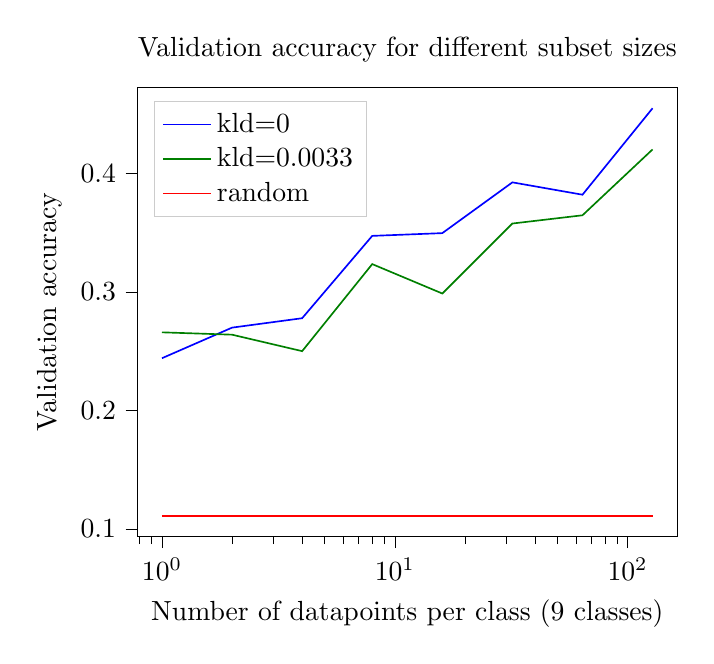
\begin{tikzpicture}
				
				\definecolor{darkgray176}{RGB}{176,176,176}
				\definecolor{green01270}{RGB}{0,127,0}
				\definecolor{lightgray204}{RGB}{204,204,204}
				
				\begin{axis}[
					legend cell align={left},
					legend style={
						fill opacity=0.8,
						draw opacity=1,
						text opacity=1,
						at={(0.03,0.97)},
						anchor=north west,
						draw=lightgray204
					},
					log basis x={10},
					tick align=outside,
					tick pos=left,
					title={Validation accuracy for different subset sizes},
					x grid style={darkgray176},
					xlabel={Number of datapoints per class (9 classes)},
					xmin=0.784584097896751, xmax=163.143760296865,
					xmode=log,
					xtick style={color=black},
					y grid style={darkgray176},
					ylabel={Validation accuracy},
					ymin=0.0939236113230387, ymax=0.472048606660631,
					ytick style={color=black}
					]
					\addplot [semithick, blue]
					table {%
						1 0.244047609737941
						2 0.26984125818525
						4 0.277777765819005
						8 0.347222211020333
						16 0.3495370165507
						32 0.392361106872559
						64 0.381944427490234
						128 0.454861106872559
					};
					\addlegendentry{kld=0}
					\addplot [semithick, green01270]
					table {%
						1 0.265873005049569
						2 0.263888875416347
						4 0.249999988419669
						8 0.323412685394287
						16 0.29861110051473
						32 0.357638893127441
						64 0.364583320617676
						128 0.420138854980469
					};
					\addlegendentry{kld=0.0033}
					\addplot [semithick, red]
					table {%
						1 0.111111111111111
						2 0.111111111111111
						4 0.111111111111111
						8 0.111111111111111
						16 0.111111111111111
						32 0.111111111111111
						64 0.111111111111111
						128 0.111111111111111
					};
					\addlegendentry{random}
				\end{axis}
				
			\end{tikzpicture}
			
			%\caption{Caption for the first graph.}
		\end{subfigure}
		\hfill
		\begin{subfigure}[b]{0.4\textwidth}
			\centering
				% graph subsets (module 2)
			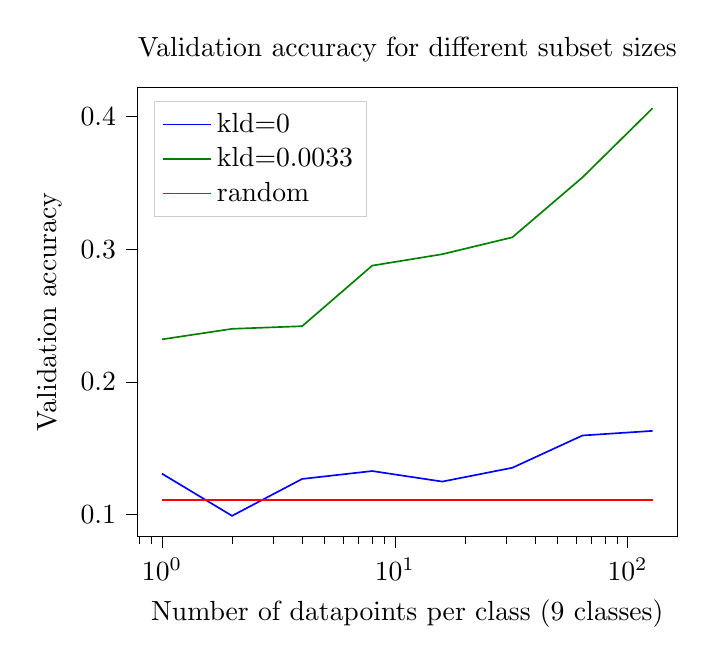
\begin{tikzpicture}
				
				\definecolor{darkgray176}{RGB}{176,176,176}
				\definecolor{green01270}{RGB}{0,127,0}
				\definecolor{lightgray204}{RGB}{204,204,204}
				
				\begin{axis}[
					legend cell align={left},
					legend style={
						fill opacity=0.8,
						draw opacity=1,
						text opacity=1,
						at={(0.03,0.97)},
						anchor=north west,
						draw=lightgray204
					},
					log basis x={10},
					tick align=outside,
					tick pos=left,
					title={Validation accuracy for different subset sizes},
					x grid style={darkgray176},
					xlabel={Number of datapoints per class (9 classes)},
					xmin=0.784584097896751, xmax=163.143760296865,
					xmode=log,
					xtick style={color=black},
					y grid style={darkgray176},
					ylabel={Validation accuracy},
					ymin=0.0838541626930237, ymax=0.421602182728904,
					ytick style={color=black}
					]
					\addplot [semithick, blue]
					table {%
						1 0.130952375956944
						2 0.0992063454219273
						4 0.126984120096479
						8 0.132936503546579
						16 0.124999993642171
						32 0.135416660308838
						64 0.159722213745117
						128 0.163194446563721
					};
					\addlegendentry{kld=0}
					\addplot [semithick, green01270]
					table {%
						1 0.23214284828731
						2 0.240079355239868
						4 0.242063480785915
						8 0.287698405129569
						16 0.296296278635661
						32 0.309027767181396
						64 0.354166641235352
						128 0.40625
					};
					\addlegendentry{kld=0.0033}
					\addplot [semithick, red]
					table {%
						1 0.111111111111111
						2 0.111111111111111
						4 0.111111111111111
						8 0.111111111111111
						16 0.111111111111111
						32 0.111111111111111
						64 0.111111111111111
						128 0.111111111111111
					};
					\addlegendentry{random}
				\end{axis}
				
			\end{tikzpicture}
			
			
			%\caption{Caption for the second graph.}
		\end{subfigure}
		\caption{Shared caption for both graphs.}
	\end{figure}


	


\section{Interpretability}

	\subsection{Decoders for Variational Greedy InfoMax}
		% investigate what info in V-GIM + argue can interpolate
		To investigate what information is contained in V-GIM's representations, we train a decoder on top of each of V-GIM's modules. Contrary to variational autoencoders, V-GIM is fully independent from the decoder and does not require one for training. Furthermore, we analyse the underlying structure the representations obtained from each module. This is achieved by altering representation's component values and observing the effects through the decoder. As we argued in the previous section, this is only possible because V-GIM's encodings is optimised to be approximate to the standard normal. As long as this is case, there are no "gaps" in the latent space around the origin. The decoder will be able to generalise to the altered representations as long as the representations are close to the origin.
		
		We train a decoder for each of V-GIM's modules. As such we can assess the information contained in the final representation, but also the representations of intermediate modules.
		
		% result:
		timesteps in second module captures much wider time frame and first module, so observes different content.
		first module: each component respoble for different frequency.
		
		second module:
		combination of frequencies.
		
		\subsubsection{Decoder architecture}
		We develop two decoders, one for each module. 
		$$
			\text{decoder}^1(\zt^1) = \xt
		$$
		$$
			\text{decoder}^2(\zt^2) = \xt
		$$
		Both decoders' architectures are symmetric to the architecture the V-GIM's encoder. Where the convolutional and max pooling layers are both replaced by transposed convolution layers.
		The architecture for 
		
		\begin{tabular}{|c|c|c|c|}
			\hline
			Layer & Filter size & Stride & Padding \\
			\hline
			TransConv1 & 3 & 1 & 1 \\
			\hline
		\end{tabular}
	
	
	
		% -----
		The decoder consists of a convolutional neural network which takes as input the encodings from V-GIM and is tasked to reconstruct the original data. The decoder is optimised to minimise the mean squared error between mel spectrograms of the original data and the reconstructed data. 
		
		We optimise the decoder with the loss function introduced in [cite] and alter it to use mel spectrograms to better capture the important speech features according to the auditory system. The loss function we use is the following:
		$$
		\mathcal{L}_{\text{decoder}} =\frac{1}{n} \sum_{i=1}^n\left( \log (MEL(y^{(i)})) -\log (MEL(\hat{y} ^{(i)} )) \right)^2
		$$
		
		
	
	
	
	
	% first module:
	
%	class SimpleV2Decoder(GimDecoder):
%	def __init__(self, hidd_channels=32, out_channels=1):
%	super().__init__("Simple_v2_DECODER")
%	
%	# Encoder architecture (Simple v2)
%	kernel_sizes = [10, 8, 3]
%	strides = [4, 3, 1]
%	padding = [2, 2, 1]
%	max_unpool_k_size = 8
%	max_unpool_stride = 4
%	
%	# Decoder architecture
%	self.decoder = nn.Sequential(
%	nn.ConvTranspose1d(hidd_channels, hidd_channels,
%	kernel_sizes[2], stride=strides[2], padding=padding[2]),
%	nn.ReLU(),
%	
%	# Replaces maxpooling
%	nn.ConvTranspose1d(hidd_channels, hidd_channels, max_unpool_k_size,
%	stride=max_unpool_stride, padding=0, output_padding=0),
%	nn.ReLU(),
%	
%	nn.ConvTranspose1d(hidd_channels, hidd_channels,
%	kernel_sizes[1], stride=strides[1], padding=padding[1], output_padding=1),
%	nn.ReLU(),
%	
%	# Replaces maxpooling
%	nn.ConvTranspose1d(hidd_channels, hidd_channels, max_unpool_k_size,
%	stride=max_unpool_stride, padding=0, output_padding=3),
%	nn.ReLU(),
%	
%	nn.ConvTranspose1d(hidd_channels, out_channels,
%	kernel_sizes[0], stride=strides[0], padding=padding[0], output_padding=2),
%	)
%	
%	def forward(self, x):
%	return self.decoder(x)
	
	
	


% Second module:
%
%class SimpleV3DecoderTwoModules(GimDecoder):
%def __init__(self, hidd_channels=32, out_channels=1):
%super().__init__("Simple_v3_2Module_DECODER")
%
%kernel_sizes = [6, 6, 3]
%strides = [2, 2, 1]
%padding = [2, 2, 1]
%
%self.module2 = nn.Sequential(
%nn.ConvTranspose1d(hidd_channels, hidd_channels,
%kernel_sizes[2], stride=strides[2], padding=padding[2]),
%nn.ReLU(),
%nn.ConvTranspose1d(hidd_channels, hidd_channels,
%kernel_sizes[1], stride=strides[1], padding=padding[1], output_padding=0),
%nn.ReLU(),
%nn.ConvTranspose1d(hidd_channels, hidd_channels,
%kernel_sizes[0], stride=strides[0], padding=padding[0], output_padding=0),
%)
%self.module1 = SimpleV2Decoder(hidd_channels, out_channels)
%
%def forward(self, z):
%z = self.module2(z)
%x = self.module1(z)  # SimpleV2Decoder
%return x

	
	
		\subsubsection{Loss function}
		
 % We use five convolutional layers with strides [5, 4, 2, 2, 2], filter-sizes [10, 8, 4, 4, 4] and 512 hidden units with ReLU activations.
	



	
	
	\subsection{Decoder: predictions on test set}
	Fig \ref{fig:bagidi1-model29-true-vs-predicted} displays the reconstructed signal from the vocal sound "ba-gi-di". The two images on the left displays the original signal, while the right two images contain the reconstructed signal.  The upper images displays the signals in time domain, the bottom images spectral domain. The reconstructed signal is an audio sample, for instance which is encoded via Greedy Infomax (up to the fourth (and final) convolution layer), this output is then given to a decoder to reconstruct the original signal.
	
	%TODO: BROKEN 
	%\begin{figure}[h]
	%	\centering
	%	\includegraphics[width=0.7\linewidth]{"../../../../../../../../../GitHub/thesis-fabian-denoodt/GIM/logs/GIM_DECODER_experiment/MSE + scFFT Loss FFT=10240 Lambda=1.0000000/lr_0.0010000/GIM_L4/predictions_model=29/test/bagidi_1, model=29, True vs Predicted"}
	%	\caption{Top left: original, time domain. Bottom left: original }
	%	\label{fig:bagidi1-model29-true-vs-predicted}
	%\end{figure}



